\section{The deuteron --- a strange fellow}
The radial schrödinger equation
\begin{equation}
	-\frac{\hbar^2}{2 m} \frac{\partial^2}{\partial r^2} u(r) + V(r) u(r) = E u(r),
\end{equation}
where $E = -B$ is the binding energy. Between $r = \SI{0}{\femto\m}$ and $r = R = \SI{2.1}{\femto\m}$ we have $V(r) = -V_0$ and thus
\begin{equation}
	\frac{\partial^2}{\partial r^2} u_\mathrm{I}(r) = -\frac{2m (V_0 - B)}{\hbar^2} u_\mathrm{I}(r),
\end{equation}
letting $k = \sqrt{2m(V_0-B)/\hbar^2}$ we get
\begin{equation}
	\frac{\partial^2}{\partial r^2} u_\mathrm{I}(r) = -k^2 u_\mathrm{I}(r) \iff u_\mathrm{I}(r) = A \sin{kr} + B \cos{kr}.
\end{equation}
For $r > R = \SI{2.1}{\femto\m}$ we have $V(r) = 0$ and thus
\begin{equation}
	\frac{\partial^2}{\partial r^2} u_\mathrm{II}(r) = \frac{2m B}{\hbar^2} u_\mathrm{II}(r),
\end{equation}
letting $q = \sqrt{2mB/\hbar^2}$ we get
\begin{equation}
	\frac{\partial^2}{\partial r^2} u_\mathrm{II}(r) = q^2 u_\mathrm{II}(r) \iff u_\mathrm{II}(r) = C e^{-qr}.
\end{equation}
For $r = \SI{0}{\femto\m}$ the wavefunction must be zero, thus
\begin{equation}
	B = 0 \implies u_\mathrm{I}(r) = A \sin{kr}
\end{equation}
Then at $r = R = \SI{2.1}{\femto\m}$ we must have $u_\mathrm{I}(R) = u_\mathrm{II}(R)$ which is
\begin{equation}
	A \sin{kR} = C e^{-qR} \iff C = \frac{\sin{kR}}{e^{-qR}}A.
\end{equation}
The wavefunction also must be normalised and thus
\begin{align}
	1 &= \int_{0}^{\infty} |u(r)|^2 \dd r = \abs{A}^2\int_{0}^{R} \abs{\sin{kr}}^2  \dd r + \abs{C}^2\int_{R}^{\infty} \abs{e^{-qr}}^2 \dd r \\
	&= \abs{A}^2 \left[   \int_{0}^{R} \sin^2{kr}\dd r + \frac{\sin^2{kR}}{e^{-2qR}} \int_{R}^{\infty} e^{-2qr} \dd r  \right] \\
	&= \abs{A}^2 \left[ \left.\left( \frac{r}{2} - \frac{\sin{2kr}}{4k}  \right)\right|_0^R  + \frac{\sin^2{kR}}{e^{-2qR}} \times \left.\left( -\frac{e^{-2qr}}{2q} \right)\right|_R^\infty  \right]\\
	&= \abs{A}^2 \left[ \frac{R}{2} - \frac{\sin{2kR}}{4k} + \frac{\sin^2{kR}}{2q}\right] \\
	&\iff A = \sqrt{\frac{1}{\frac{R}{2} - \frac{\sin{2kR}}{4k} + \frac{\sin^2{kR}}{2q}}}
\end{align}
Calculating this numerically with python gives $A = 0.56$ and $C = 0.87$. By integrating $|u(r)|^2$ we can find the probability of the distance being greater than \SI{2.1}{\femto\m}. That is we want to calculate
\begin{equation}
	P(r > \SI{2.1}{\femto\m}) = \int_{\SI{2.1}{\femto\m}}^\infty |u(r)|^2 \dd r.
\end{equation}
Using python we get a probability of $P(r > \SI{2.1}{\femto\m}) = \SI{62.2}{\percent}$.

\begin{figure}[H]
	\centering
	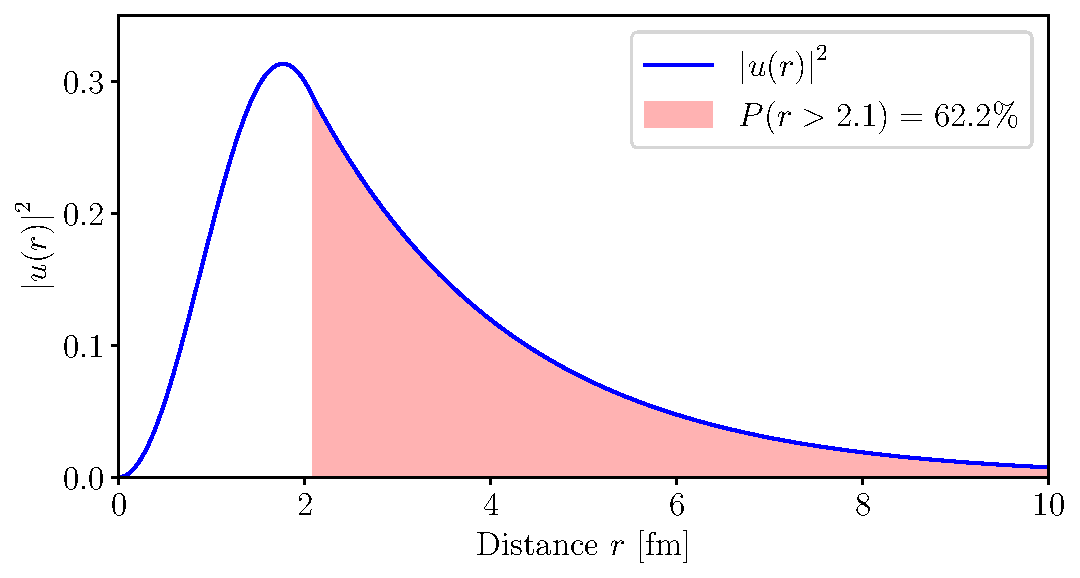
\includegraphics[width=\textwidth]{./code/Exercise4.pdf}
	\caption{The probability distribution of the deuteron.}
\end{figure}

\paragraph{Answer:} The deuteron spend \SI{62.2}{\percent} of the time beyond their nuclear force range.